\section{Diffusion-Reaction Equation With Forced Current through the system.}

We consider the same system as above

\begin{align}
	\frac{\partial C}{\partial t} = \frac{\partial^2 C}{\partial x^2},
\end{align}

with a slight change in border conditions. We want to impose the current on the system, which should be proportional to the reaction rate at the interface.

\begin{align}
	R &= k_f C(0^+, t)\\ 
	&= \frac{i_0}{\mathcal{F}}.
\end{align}

This yields the following border and initial conditions for the problem

\begin{align}
	C(\delta, t) &= C_b,\\
	C(0^+, t) &= \frac{R}{k_f},\\
	C(x, 0) &= 0.
\end{align}

or equivalently

\begin{align}
	C(\delta, t) &= C_b,\\
	C(0^+, t) &= \frac{i_0}{\mathcal{F}k_f},\\
	C(x, 0) &= 0.
\end{align}

\subsection{Steady State Solution}

As always, first we compute the steady state solution.

\begin{align}
	\frac{d ^2C}{d x^2} = 0.
\end{align}

The solution is of the form

\begin{align}
	C_{SS}(x) = A + Bx.
\end{align}

Border conditions yield,

\begin{align}
	C_{SS}(\delta) &= A + B\delta\\
	&= C_b,
\end{align}

and

\begin{align}
	C_{SS}(0) &= A \\
	&= \frac{i_0}{\mathcal{F} k_f}.
\end{align}

Therefore,

\begin{align}
	C_{SS} (x) = \frac{i_0}{\mathcal{F}k_f} +\qty{C_b - \frac{i_0}{\mathcal{F}k_f}}\frac{x}{\delta}
\end{align}

\subsection{Dynamic Solution}

To solve the dynamic solution, we consider the following change of variable

\begin{align}
	\rho(x, t) = \frac{C(x,t)-C_{SS}(x)}{C_b}.
\end{align}

As in previous sections, we define the dimensionless parameters $\tau = \frac{\mathcal{D} t}{\delta^2}$, $\xi = \frac{x}{\delta}$. This leads to the equation

\begin{align}
	\frac{\partial \rho}{\partial \tau} = \frac{\partial^2 \rho}{\partial \xi^2}.
\end{align}

Let $\rho(\xi, \tau)$ be of the form

\begin{align}
	\rho(\xi, \tau) = F(\xi)G(\tau).
\end{align}


Separation of variables leads to the Sturm-Liouville problem

\begin{align}
	\frac{d G}{d \tau} + \lambda^2G(\tau) = 0,
	\label{eq:G-eq}\\
	\frac{d^2 F}{d\xi^2} + \lambda^2 F(\xi) = 0.
	\label{eq:F-eq}
\end{align}


The solution of \ref{eq:G-eq} is 

\begin{align}
	G(\tau) = G(0) e^{-\lambda^2 \tau},
\end{align}

whereas for \ref{eq:F-eq} we get the particular solution,

\begin{align}
	F(\xi) = A_\lambda\sin(\lambda \xi) + B_\lambda\cos(\lambda \xi)
\end{align}

Border conditions yield 

\begin{align}
	B = 0,\\
	\lambda = n\pi.
\end{align}

where $n$ is an integer number. We let $A_n = G(0) A_\lambda$ and the general solution for $\rho$ is

\begin{align}
	\rho(\xi, \tau) = \sum_n A_n e^{-n^2\pi^2 \tau}\sin(n\pi \xi)
\end{align}


Consider the following integral

\begin{align}
	J_{n,m} = \int_0^1 \sin(n\pi\xi) \sin(m\pi\xi) d\xi.
\end{align}

It can be shown that 

\begin{align}
	J_{n,m} = \frac{1}{2}\delta_{n,m}.
	\label{eq:jnm}
\end{align}

Using \ref{eq:jnm}, we can compute the value of $A_n$ using the initial condition,

\begin{align}
	\rho(\xi, 0) &= \sum_n A_n \sin(n\pi\xi)\\
	 &= -\frac{C_{SS}(\xi)}{C_b}.
\end{align}

or equivalently,

\begin{align}
	A_n = -\frac{2}{C_b} \int_0^1 C_{SS}(\xi)\sin(n\pi\xi) d\xi
\end{align}

Computing the integral and using \ref{eq:steady-state} we get

\begin{align}
	A_n = -\frac{2}{n\pi C_b} \qty{\frac{i_0}{k_f\mathcal{F}} - (-1)^n C_b}.
\end{align}


Therefore,

\begin{align}
	\rho(\xi, \tau) = \sum_n \frac{2}{n\pi C_b} \qty{(-1)^n C_b- \frac{i_0}{k_f\mathcal{F}}} e^{-n^2\pi^2\tau}\sin(n\pi\xi)
\end{align}


Therefore,

\begin{align}
	C(\xi, \tau) = \frac{i_0}{\mathcal{F}k_f} +\qty{C_b - \frac{i_0}{\mathcal{F}k_f}}\xi +\frac{2}{\pi}\sum_n \qty{(-1)^n C_b- \frac{i_0}{k_f\mathcal{F}}} \frac{e^{-n^2\pi^2\tau}}{n}\sin(n\pi\xi)
\end{align}


\begin{figure}[htbp]
\centering
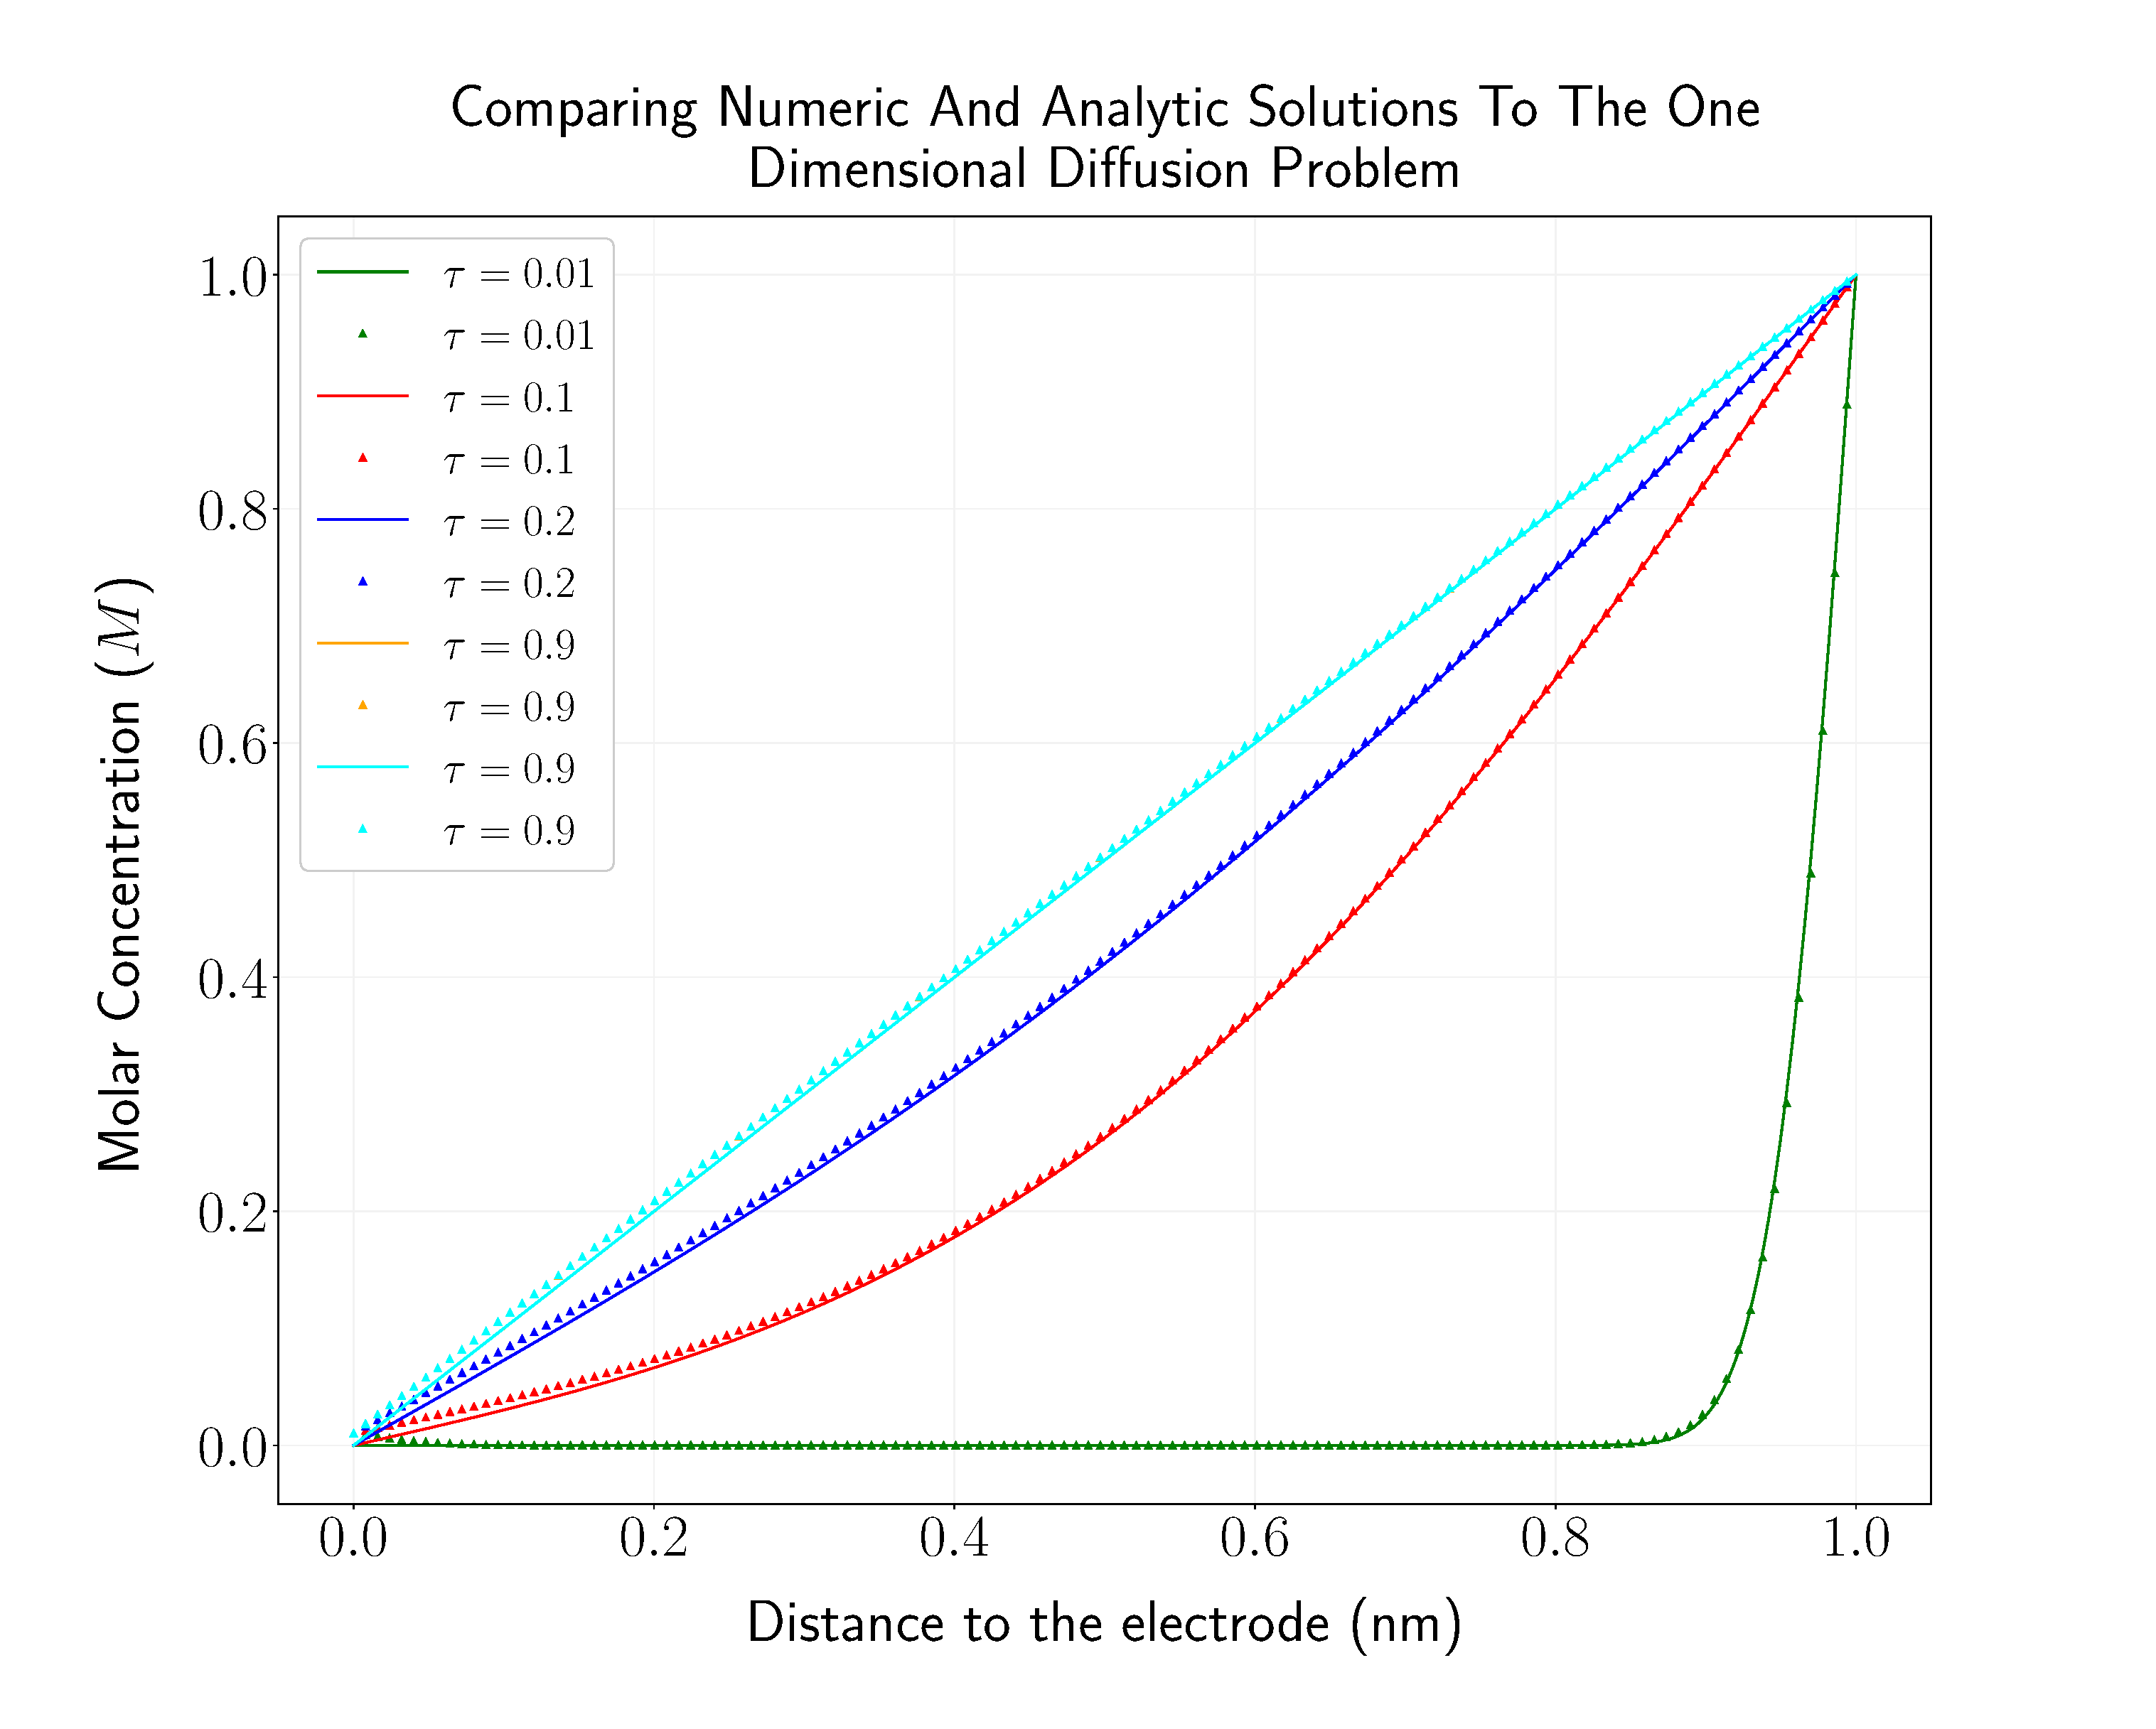
\includegraphics[width=\textwidth]{forced-current-dynamic.eps}
\caption{}
\label{fig:diffusion-reaction-comparison}
\end{figure}
